
\chapter{Modelo de Datos}
\section{Requisitos}\label{requisitos}
A continuación se establecen los requisitos del sistema de datos solicitado por la universidad.
\begin{enumerate}
  \item\label{linea1} Cada profesor tiene RUN, nombre, edad, rango y especialidad de investigación.
  \item\label{linea2} Cada proyecto tiene número de proyecto, nombre de patrocinador (por ejemplo, el CSIC), fecha de comienzo, fecha de finalización y presupuesto.
  \item\label{linea3} Cada alumno tiene RUN, nombre, edad.
  \item\label{linea4} Cada alumno puede o no pertenecer a un programa de postgrado (por ejemplo, magíster o doctorado), del cual interesa el nombre y código.
  \item\label{linea5} Cada proyecto está dirigido por un profesor (conocido como investigador principal de ese proyecto).
  \item\label{linea6} En cada proyecto trabajan uno o varios profesores (conocidos como investigadores de ese proyecto).
  \item\label{linea7} Cada profesor puede dirigir varios proyectos o trabajar en ellos.
  \item\label{linea8} En cada proyecto trabajan uno o varios alumnos de postgrado (conocidos como ayudantes de investigación de ese proyecto).
  \item\label{linea9} Cuando los alumnos de postgrado trabajan en un proyecto, su trabajo debe supervisarlo un profesor. Cada alumno de postgrado puede trabajar en varios proyectos, en cuyo caso puede tener un supervisor diferente en cada uno de ellos.
  \item\label{linea10} Cada departamento tiene número de departamento, nombre de departamento y despacho principal.
  \item\label{linea11} Cada departamento tiene un profesor (conocido como director) que lo dirige.
  \item\label{linea12} Cada profesor trabaja en uno o varios departamentos, y por cada departamento en que trabaja se asocia un porcentaje de tiempo a su trabajo.
  \item\label{linea13} Cada alumno de postgrado tiene un departamento principal en el que trabaja en su titulación.
  \item\label{linea14} Cada alumno de postgrado tiene otro alumno de postgrado más veterano (conocido como asesor del alumno) que lo aconseja sobre las asignaturas en las que debe matricularse.
  
\end{enumerate}
\section{Modelo Entidad Relación}
\subsection{Definición de Entidades}\label{s:defentidad}

\subsubsection{Herencia}

A partir de los requisitos expuestos en las líneas \ref{linea1} y \ref{linea2}, se identifican las entidades \texttt{Pro\-fe\-sor} y \texttt{Alumno}. Ambas comparten atributos inherentes al concepto de \texttt{Persona}, por lo que se propone utilizar una jerarquía de herencia para optimizar el modelo de datos, como se ilustra en la Figura \ref{f:hpersona}. Dado que los únicos roles definidos en el sistema son \texttt{Profesor} y \texttt{Alumno}, y no se contempla la posibilidad de que un individuo ocupe ambos roles simultáneamente, se define esta especialización como \textbf{total y sin solapamiento}. Esto implica que cada instancia de \texttt{Persona} registrada en el sistema será exclusivamente un \texttt{Profesor} o un \texttt{Alumno}.


\begin{figure}[H]
\centering
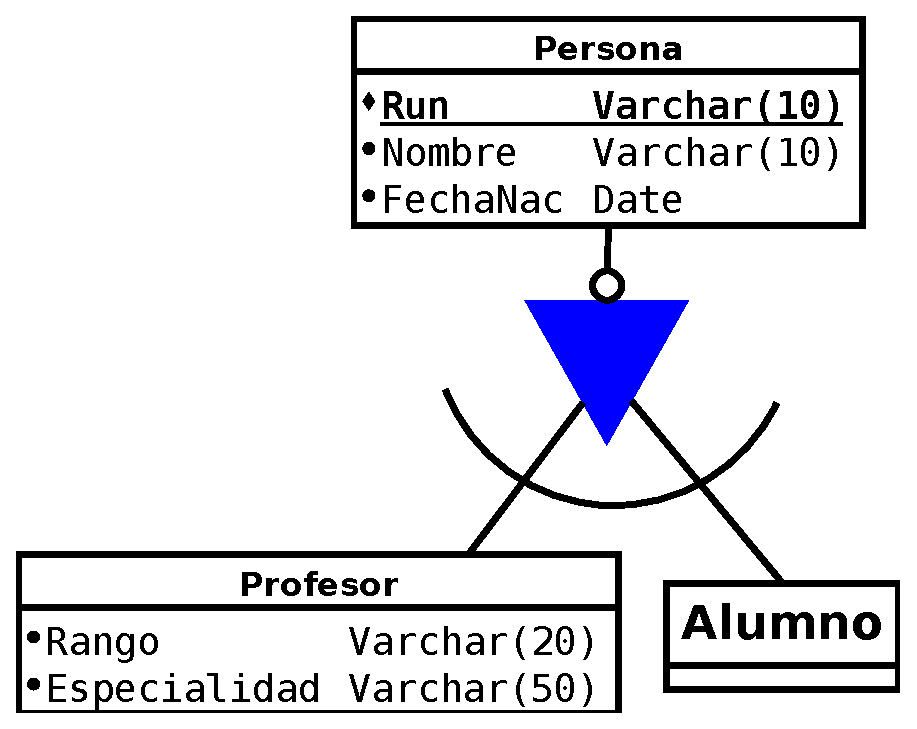
\includegraphics[width=0.5\textwidth]{images/MER/MER_Universidad2_Herencia.eps}
    \caption{Herencia Persona}
    \label{f:hpersona}
\end{figure}

\subsubsection{Entidades individuales}
A partir del requisito de la línea \ref{linea2}, se define la entidad \texttt{Proyecto}. La estructura detallada de esta entidad, incluyendo sus atributos y características, se presenta en la Tabla \ref{tab:eproyecto}.

\begin{table}[H]
    \centering
    \begin{tabular}{|ll|}\hline
        \multicolumn{2}{|c|}{\textbf{Proyecto}}\\\hline
        \textbf{Numero} (PK)& Integer\\
        Patrocinador& Varchar (20)\\
        FechaInicio&Date\\
        FechaFin&Date\\
        Presupuesto&Money\\
        \hline
    \end{tabular}
    \caption{Entidad Proyecto}
    \label{tab:eproyecto}
\end{table}

El requerimiento expuesto en la línea \ref{linea4} da origen a la entidad \texttt{Postgrado}, cuya composición y atributos se desglosan en la Tabla \ref{tab:epostgrado}.

\begin{table}[H]
    \centering
    \begin{tabular}{|ll|}\hline
        \multicolumn{2}{|c|}{\textbf{Postgrado}}\\\hline
        \textbf{Codigo} (PK)& Integer\\
        Nombre& Varchar (30)\\
        \hline
    \end{tabular}
    \caption{Entidad Postgrado}
    \label{tab:epostgrado}
\end{table}


La entidad \texttt{Departamento}, identificada a partir del requerimiento de la línea \ref{linea10}, se detalla en la Tabla \ref{tab:edepartamento}, donde se especifican sus atributos y características.

\begin{table}[H]
    \centering
    \begin{tabular}{|ll|}\hline
        \multicolumn{2}{|c|}{\textbf{Departamento}}\\\hline
        \textbf{Numero} (PK)& Integer\\
        Nombre& Varchar (30)\\
        Despacho&Integer\\\hline
    \end{tabular}
    \caption{Entidad Departamento}
    \label{tab:edepartamento}
\end{table}


%\subsubsection{Conjunto de Entidades}
%El conjunto de todas las entidades principales de este proyecto son las presentes en la Figura \ref{f:entidades}.


\subsection{Definición de Relaciones}\label{s:defrelacion}
\subsubsection{Relaciones n-aria}

A partir de los requisitos de las líneas \ref{linea6} y \ref{linea9}, se define la relación ternaria \texttt{Supervisar} que vincula a \texttt{Profesor}, \texttt{Alumno} y \texttt{Proyecto} (ver Figura \ref{f:mersupervisar}). Aunque un profesor puede supervisar a varios alumnos y un proyecto puede involucrar a muchos, el requisito \ref{linea9} impone una restricción clave: la supervisión de un alumno en un proyecto específico es realizada por un único profesor. Esto refina la cardinalidad general, estableciendo una dependencia funcional donde el par (\texttt{Alumno}, \texttt{Proyecto}) determina al \texttt{Profesor} supervisor.

\begin{figure}[H]
\centering
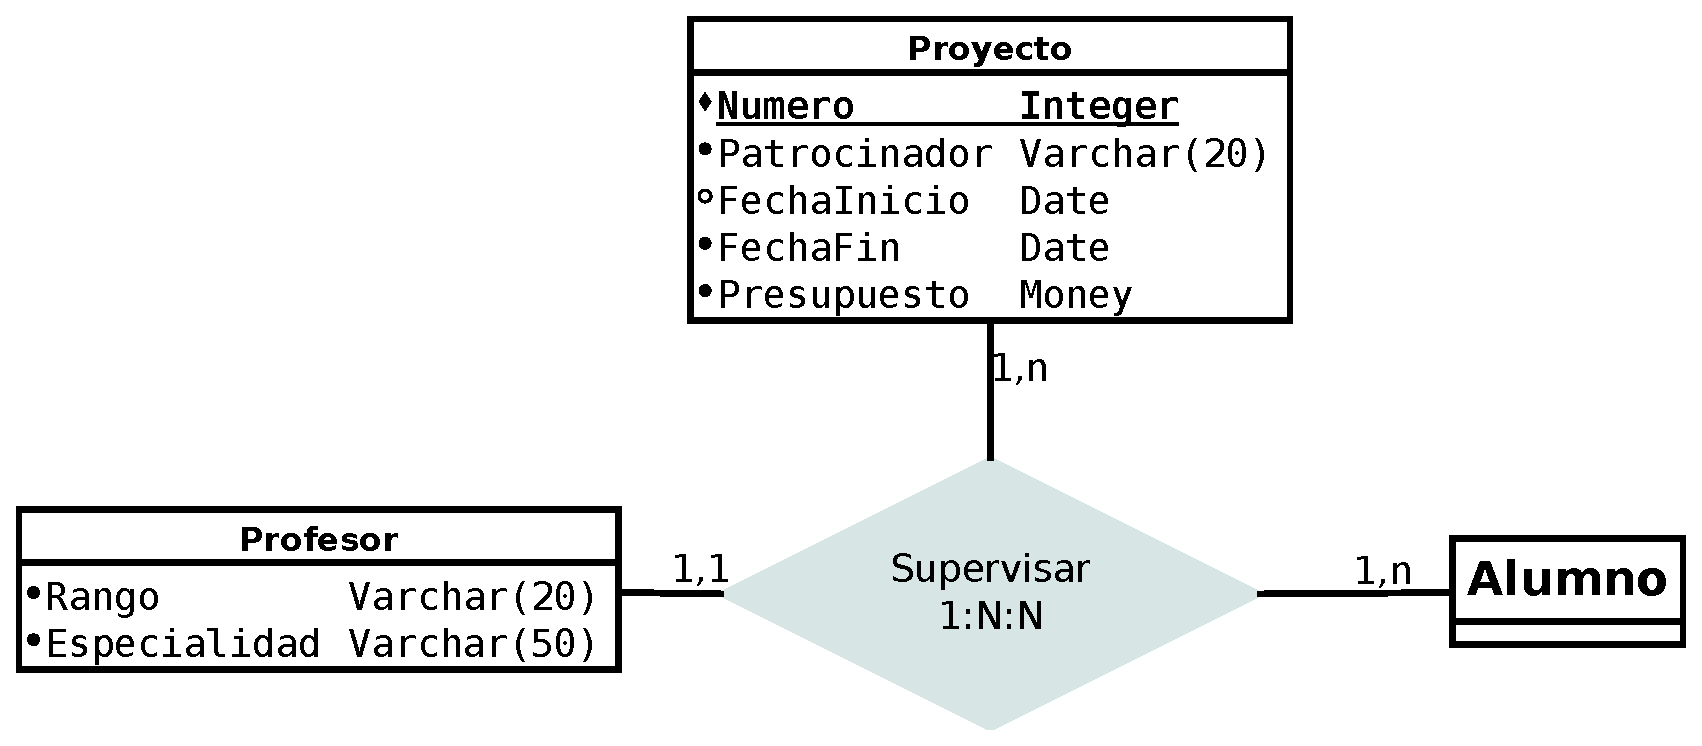
\includegraphics[width=0.8\textwidth]{images/MER/supervisar_nan.eps}
    \caption{Relación Supervisar}
    \label{f:mersupervisar}
\end{figure}

\subsubsection{Relaciones Muchos a Muchos (N:N)}

Si bien el requisito de la línea \ref{linea5} sugiere que un proyecto es dirigido por 'un' profesor, para dotar al sistema de mayor flexibilidad y capacidad a futuro, se opta por modelar la relación \texttt{Dirigir} como muchos a muchos (N:M). Esta decisión de diseño, ilustrada en la Figura \ref{f:merdirigir}, permite que el sistema registre múltiples directores o co-directores por proyecto si fuera necesario, cumpliendo a la vez con el requisito de la línea \ref{linea7} que establece que un profesor puede dirigir varios proyectos. Este enfoque proporciona mayor adaptabilidad a casos de uso complejos.

\begin{figure}[H]
\centering
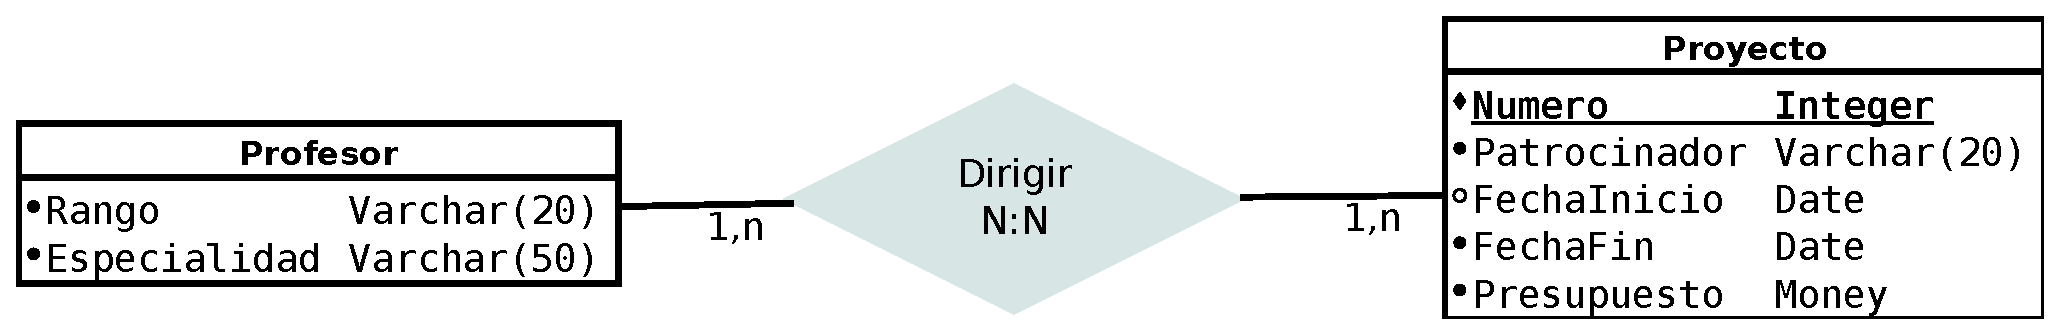
\includegraphics[width=0.8\textwidth]{images/MER/dirigir_nan.eps}
    \caption{Relación Dirigir}
    \label{f:merdirigir}
\end{figure}


El requisito de la línea \ref{linea12} establece que un profesor puede trabajar en varios departamentos y que a esta vinculación se le asocia un ``porcentaje de tiempo''. Para modelar esto correctamente, se define la relación \texttt{Laborar} con una cardinalidad de muchos a muchos (N:M) entre \texttt{Profesor} y \texttt{Departamento}. Esta relación, ilustrada en la Figura \ref{f:merlaborar}, incluye el atributo \texttt{porcentaje} que depende de la combinación de un profesor y un departamento específicos.

\begin{figure}[H]
\centering
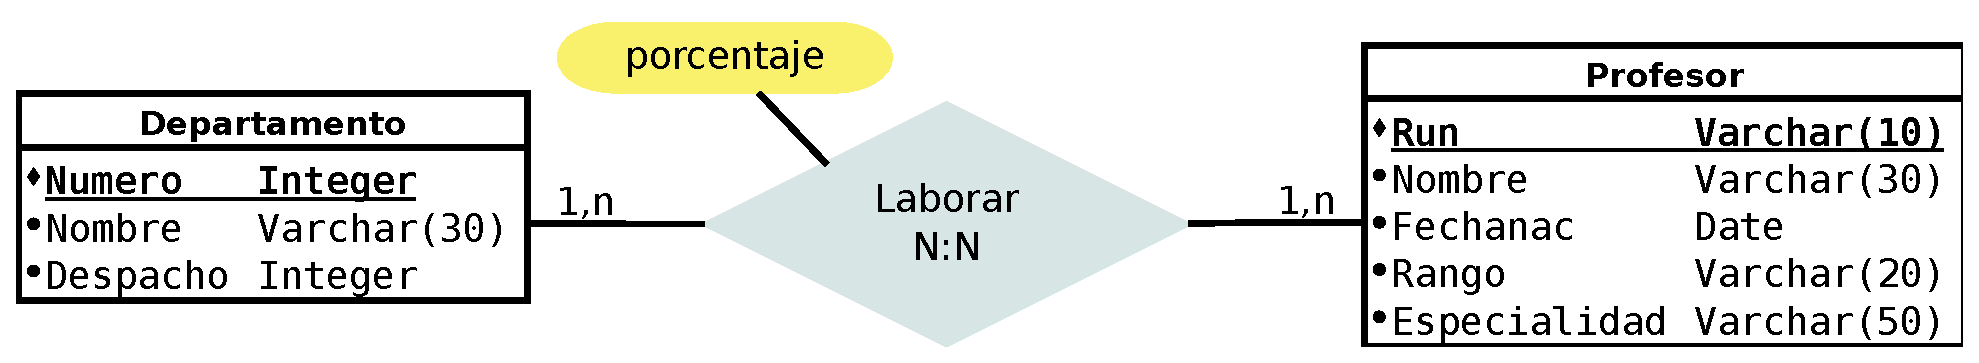
\includegraphics[width=0.8\textwidth]{images/MER/laborar_nan.eps}
    \caption{Relación Laborar}
    \label{f:merlaborar}
\end{figure}

A partir del requisito expuesto en la línea \ref{linea8}, se establece la relación \texttt{Trabajar} entre las entidades \texttt{Proyecto} y \texttt{Alumno}. Se trata de una relación con cardinalidad muchos a muchos (N:M), ya que un proyecto puede tener ``uno o varios'' alumnos trabajando en él, y (como se complementa en la línea \ref{linea9}) un alumno puede trabajar en varios proyectos (Ver Figura \ref{f:mertrabajar}).

\begin{figure}[H]
\centering
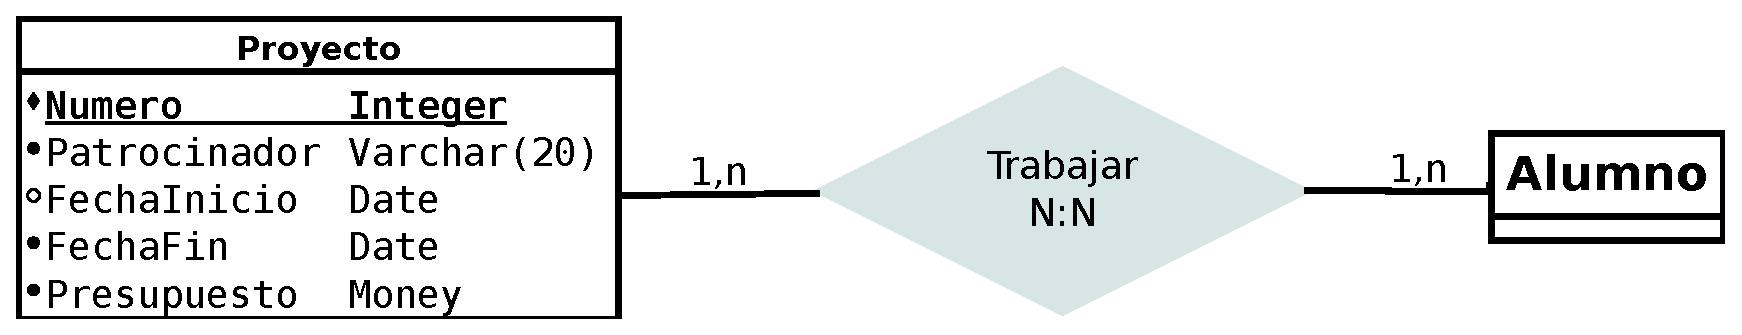
\includegraphics[width=0.8\textwidth]{images/MER/trabajar_nan.eps}
    \caption{Relación Trabajar}
    \label{f:mertrabajar}
\end{figure}


\subsubsection{Relaciones Uno a Muchos (1:N)}
La relación \texttt{Cursar}, que vincula a un \texttt{Alumno} con un \texttt{Postgrado}, se deriva del requisito de la línea \ref{linea4}. Este define una cardinalidad de uno a muchos (1:N), donde un \texttt{Postgrado} puede tener múltiples alumnos inscritos, pero un \texttt{Alumno} solo puede pertenecer a un programa de postgrado a la vez, siendo esta participación opcional. La Figura \ref{f:mercursar} ilustra esta relación y sus respectivas cardinalidades (0,1) para \texttt{Alumno} y (0,N) para \texttt{Postgrado}.

\begin{figure}[H]
\centering
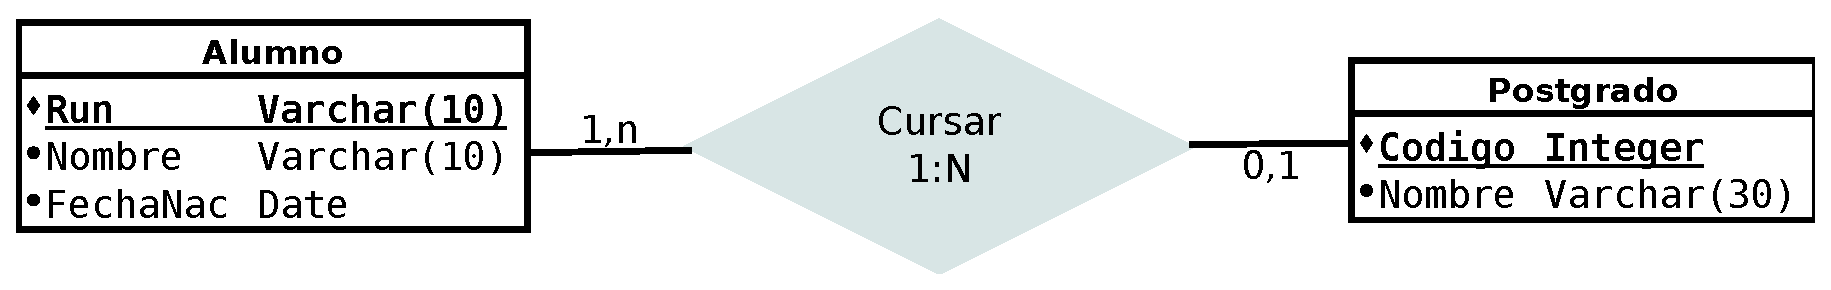
\includegraphics[width=0.8\textwidth]{images/MER/cursar_1an.eps}
    \caption{Relación Cursar}
    \label{f:mercursar}
\end{figure}

A partir del requisito de la línea \ref{linea13}, se define la relación \texttt{Pertenece} como una asociación de uno a muchos (1:N) que vincula a \texttt{Departamento} con \texttt{Alumno}. Como se ilustra en la Figura \ref{f:merpertenecer}, esta cardinalidad refleja que, si bien un departamento puede tener múltiples alumnos (1,N), cada alumno de postgrado debe estar asociado obligatoriamente a un único departamento principal (1,1).
\begin{figure}[H]
\centering
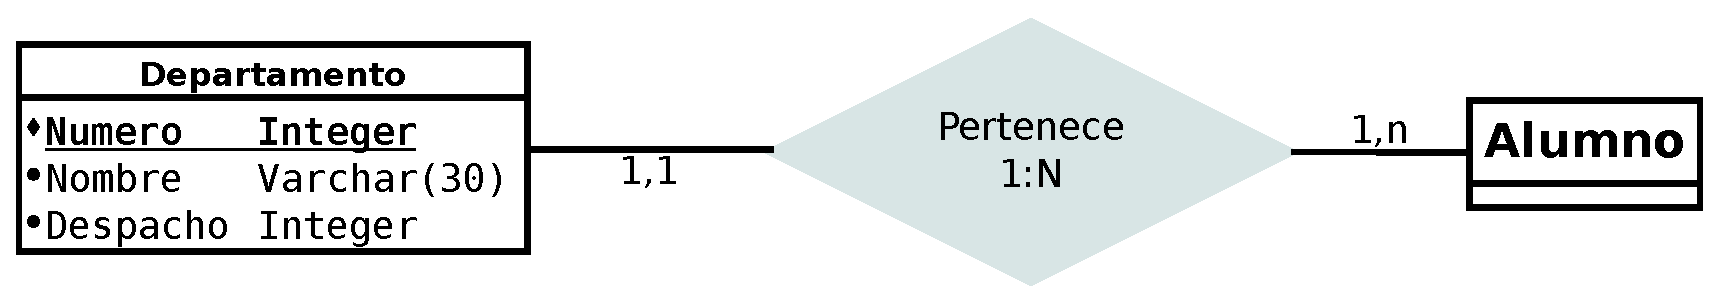
\includegraphics[width=0.8\textwidth]{images/MER/pertenece_1an.eps}
    \caption{Relación Pertenece}
    \label{f:merpertencer}
\end{figure}

\subsubsection{Relaciones Uno a Uno (1:1)}
A partir del requisito de la línea \ref{linea11}, se define la relación \texttt{Administrar} como una asociación de uno a uno (1:1) que vincula a un \texttt{Departamento} con su \texttt{Profesor} director. La Figura \ref{f:meradministrar} ilustra esta estructura, donde la participación del \texttt{Departamento} es obligatoria y única (1,1), mientras que la del \texttt{Profesor} en este rol es opcional y, como máximo, única (0,1).
\begin{figure}[H]
\centering
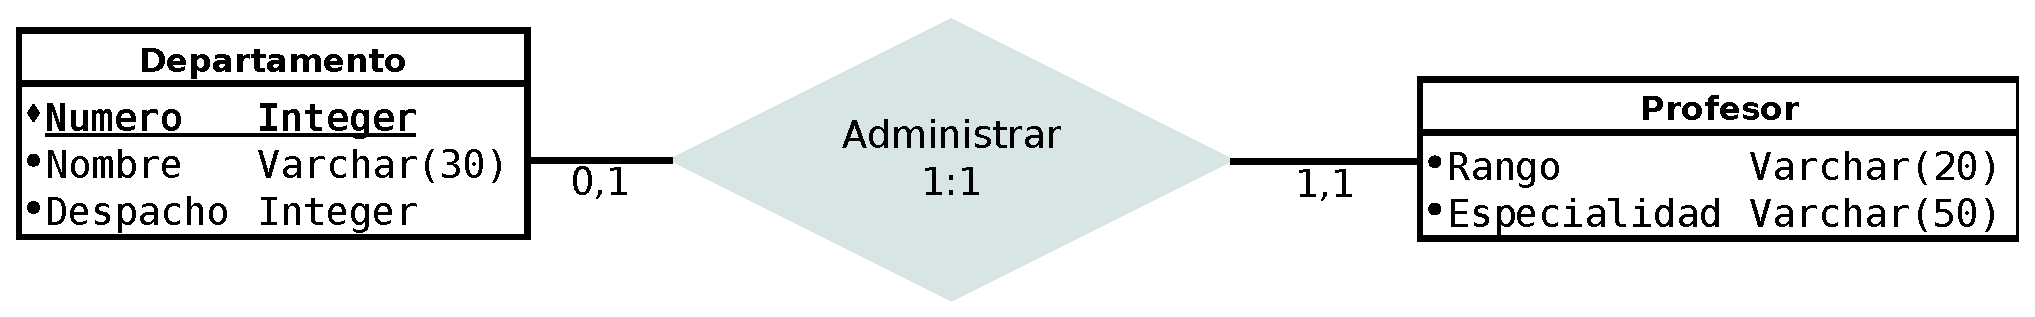
\includegraphics[width=0.8\textwidth]{images/MER/administrar_1a1.eps}
    \caption{Relación Administrar}
    \label{f:meradministrar}
\end{figure}

\subsubsection{Relaciones Reflexivas}
El requisito de la línea \ref{linea14}, que establece que cada alumno tiene un asesor más veterano, da origen a la relación reflexiva \texttt{Asesorar} en la entidad \texttt{Alumno}. Se trata de una relación de uno a muchos (1:N), donde un alumno en el rol de "asesor" puede guiar a múltiples alumnos "asesorados", mientras que cada asesorado está vinculado obligatoriamente a un único asesor. Esta estructura recursiva se representa en la Figura \ref{f:merasesorar}.

\begin{figure}[H]
\centering
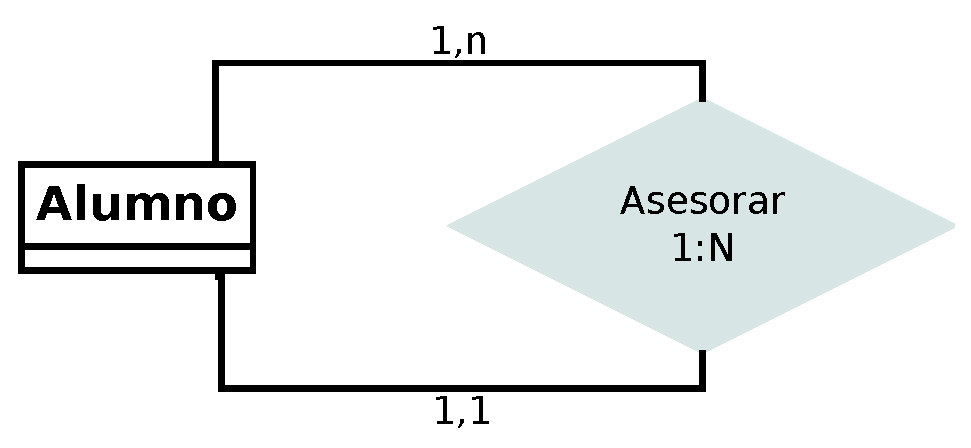
\includegraphics[width=0.6\textwidth]{images/MER/asesorar_1an.eps}
    \caption{Relación Asesorar}
    \label{f:merasesorar}
\end{figure}


\begin{landscape}
\subsection{Modelo Entidad Resultante}
Una vez establecidas las entidades y sus atributos como se presentó en la sección \ref{s:defentidad} y las relaciones y herencia presentadas en la sección \ref{s:defrelacion}, se obtiene el modelo Entidad Relación completo que se ve en la Figura \ref{f:mer}.
\begin{figure}[htb]
\centering
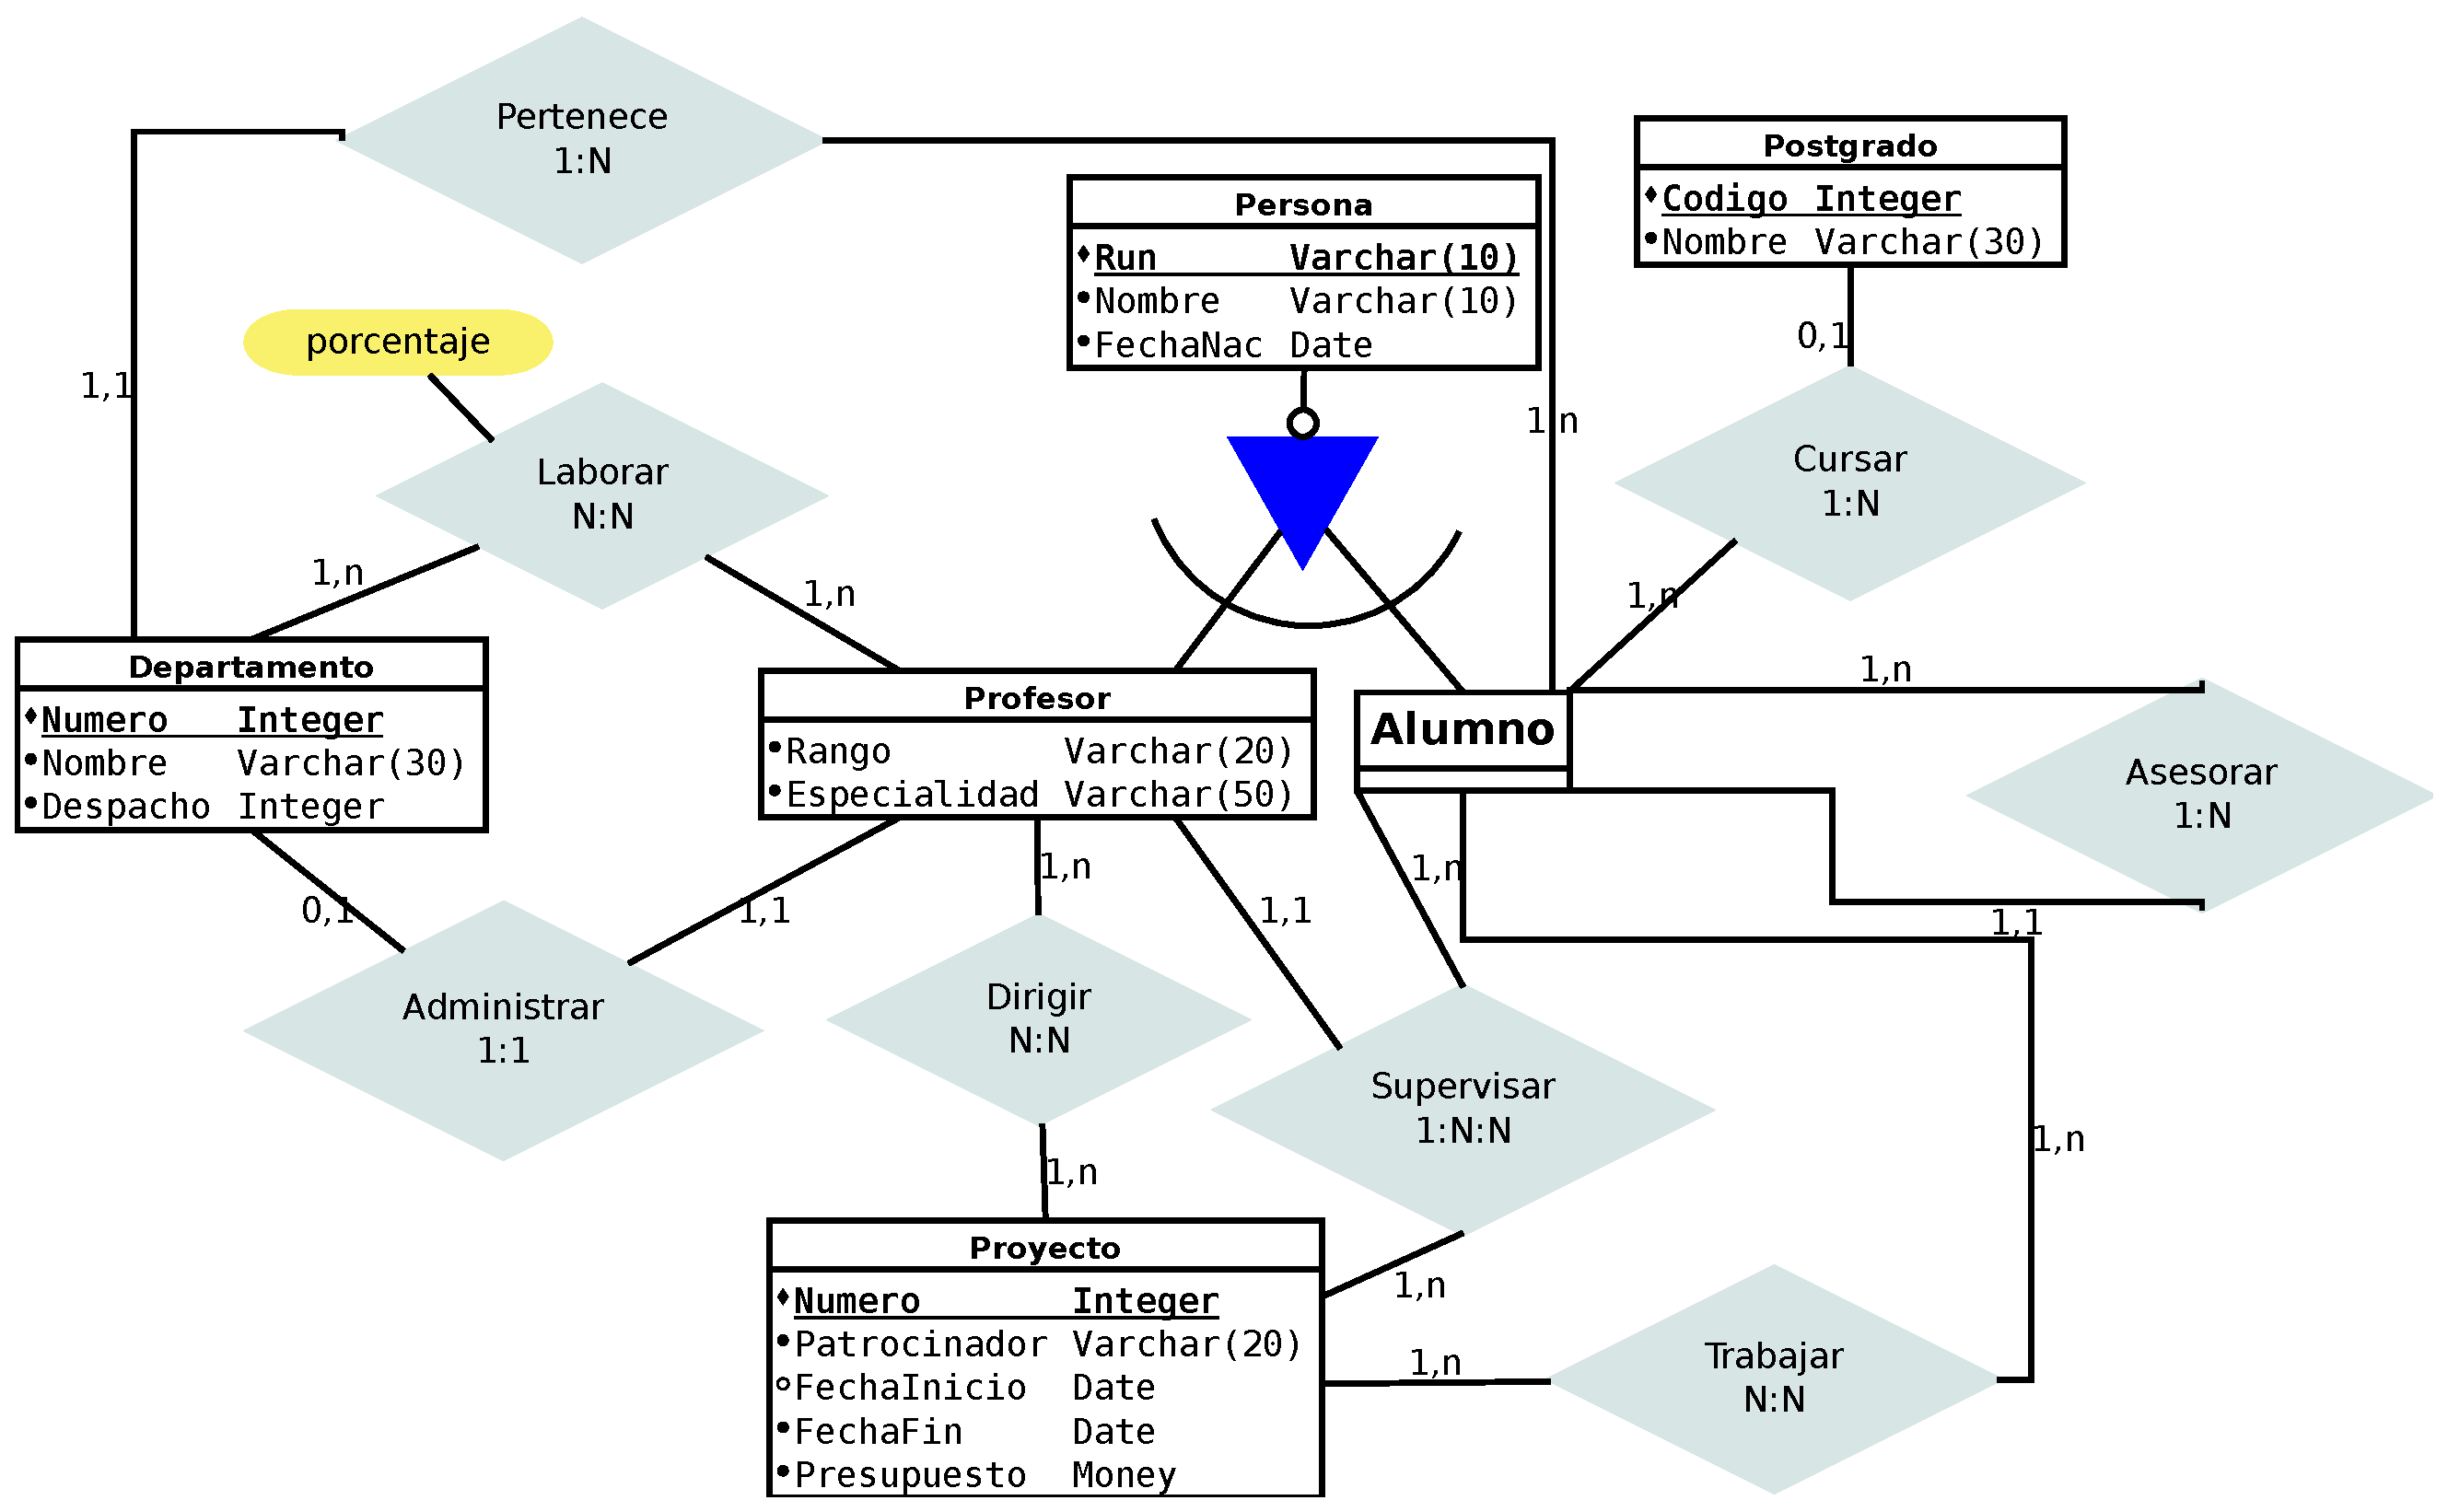
\includegraphics[width=1.15\textwidth]{images/MER/MER_Universidad2_cH.eps}
    \caption{Modelo Entidad Relación de la universidad}
    \label{f:mer}
\end{figure}
\end{landscape}

\begin{landscape}
\subsection{Modelo Entidad Relación sin Herencia}
Considerando el Modelo Entidad Relación de la Figura \ref{f:mer} se aprecia que se implementó una herencia total sin solapamiento, lo que implica que para eliminarla se debe hacer eliminación del supertipo, por lo que los atributos del padre como sus relaciones pasan ahora a las entidades hijas, con esto obtenemos el modelo entidad relación final que se ve en la Figura \ref{f:mersh}.

\begin{figure}[htb]
\centering
\includegraphics[width=1.2\textwidth]{images/MER/MER_Universidad2_sH.eps}
        \caption{MER de la universidad aplicado Eliminación del supertipo a la herencia}
    \label{f:mersh}
\end{figure}


\end{landscape}

